\documentclass{jlreq}

\usepackage{amsmath}
\usepackage{bm}
\usepackage{fancyhdr}
\usepackage{float}
\usepackage{graphicx}
\usepackage{physics}
\usepackage{siunitx}

\numberwithin{equation}{section}

\pagestyle{fancy}
\fancyhf{}
\fancyhead[R]{\thepage}

\begin{document}

\tableofcontents
\clearpage

\section{分析的評価の目的}
ATM\_Aの分析的評価を行い,個人の評価と班員の評価を比べることで問題点を抽出する.また,その問題点を基に具体的な解決策を考えて再設計する.

\section{実験機材}
使用した機材は,Dell\ Inspiron\ 15\ 3535である.OSはWindows11\ Homeであり,用いたR言語はR\ version\ 4.3.2である.

\section{分析的評価の方法}
銀行ATMのインターフェースのプロトタイプであるATM\_Aを実施してログを取得した.そのインターフェースを,Nelsenの10項目を基に評価した.
その後,評価内容を班員全員と共有し,問題点を炙り出した.また,問題点について考察を行い,評価をもとに要求獲得と再設計を行い,実装を行った.

\section{分析的評価の結果}
ATM\_Aの分析的評価の結果を,個人の結果は表\ref{tab:eval_personal}に,班員の評価は表\ref{tab:eval_group}に示す.

\begin{table}[H]
  \centering
  \caption{ATM\_Aの分析的評価(個人)}
  \scalebox{0.4}{\begin{tabular}{|l|l|}
      \hline
      1 システムの状態を視認できるようにする                   & ・現在位置を表示すべき                                                                   \\ \hline
      \begin{tabular}{l}
        2 実環境にあったシステムを構築する                 \\
        (専⾨⽤語は避け,ユーザが普段使う⾔葉を使⽤する) \\
      \end{tabular}    & ~                                                                                                  \\ \hline
      3 ユーザにコントロールの主導権と自由度を与える           & ~                                                                                        \\ \hline
      4 操作と表示に一貫性を持たせる                          & \begin{tabular}{l}
                                                                   ・テンキーやかな入力は,昇順やかな順になるように一貫性を持たせて表示すべき.             \\
                                                                   ・ボタンの色が薄かったり,濃かったり統一されていないのと,薄い表示のときに認識しづらい. \\
                                                                   ・名前の一覧表示では,あかさたな順でそれぞれまとめた方が見やすい.                       \\
                                                                 \end{tabular} \\ \hline
      5 フィードバックを与え、エラーの発生を事前に防止する     & ・振込金額を指定していなくても,フィードバックなしに確定できてしまう.                   \\ \hline
      6 記憶の負担を最小限にし、見た目だけで分かるようにする。 & ・ボタンの色が全部一緒なので,ボタンの識別が難しい.                                     \\ \hline
      7 柔軟性と効率性を持たせる(ショートカットなど)。         & \begin{tabular}{l}
                                                                   ・いくつか前の操作画面に戻るには,何回か戻るボタンを押す必要があるが, \\
                                                                   操作画面を選択することでそのページまで飛べるようにしたい.             \\
                                                                   ・1文字削除できる機能が欲しい.                                        \\
                                                                 \end{tabular}                   \\ \hline
      8 余分な情報を提示しない最小限で美しいデザインにする。   & \begin{tabular}{l}
                                                                   金融機関名が一覧表示になっているが,「あ」から始まる金融機関名などのように, \\
                                                                   あかさたなグループにして表示するべき.
                                                                 \end{tabular}             \\ \hline
      9 ユーザがエラーを認識し、回復できるようにする。         & ~                                                                                        \\ \hline
      10 ヘルプやマニュアルを用意する。                        & ~                                                                                        \\ \hline
    \end{tabular}}
  \label{tab:eval_personal}
\end{table}

\begin{table}[H]
  \centering
  \caption{ATM\_Aの分析的評価(自分を除く班全員)}
  \scalebox{0.15}{\begin{tabular}{|l|l|l|l|l|l|l|}
      \hline
      ヒューリスティック評価                                   & 31                                                                                                & 32                                                                         & 33左                                                                                                          & 33右 & 34                                           & 35 \\ \hline
      1 システムの状態を視認できるようにする                   & 現在の項目は文字を読めばわかるが分かりにくい。わかりやすく表示するべき。                          & ~                                                                          & 〇 (現在位置を表示するべきである。)                                                                          & ~    & ~                                            & ~  \\ \hline
      \begin{tabular}{l}
        2 実環境にあったシステムを構築する \\
        (専⾨⽤語は避け,ユーザが普段使う⾔葉を使⽤する)
      \end{tabular}       & \begin{tabular}{l}
                              専門用語はない。取り消しという言葉が項目を全てキャンセルして \\
                              ホームに戻っているので別の言葉を使うべき
                            \end{tabular}                                   & ~                                                                          & ☆ (分からないものは"?"のようなボタンを用意し, その場で回答を得られるようにするべきである。)                  & ~    & ~                                            & ~                                                                                         \\ \hline
      3 ユーザにコントロールの主導権と自由度を与える           & 振込先の銀行がその他で区切られているのが分かりづらくなることもありそう                            & 支店選びをカタカナ入力からだけでなく一覧から選択することができてもよさそう & ~                                                                                                             & ~    & ・「取り消し」と「戻る」の違いが分かりにくい & ~  \\ \hline
      4 操作と表示に一貫性を持たせる                          & 取り消しボタンが表示する画面で違う。数字、カタカナの並びも不規則でわかりづらい                    & 取り消しのボタンの位置が途中で変わる                                       & \begin{tabular}{l}
                                                                                                                                                                                                                                                    ☆ 表の項目行とボタンの座標がほぼ同じで、それぞれの座標が対応する行に対する操作であると誤解させかねない。 \\
                                                                                                                                                                                                                                                    △ 数字をキーボードで入力しても表示されることはよくない(おそらく、テキストボックスの機能上、訂正できないが)。
                                                                                                                                                                                                                                                  \end{tabular} & ~    & ~                                            & \begin{tabular}{l}
                                                                                                                                                                                                                                                                                                                          ・振込先の支店名頭文字入力のおいて、規則性がなく視認しづらい               \\
                                                                                                                                                                                                                                                                                                                          ・振込先の口座番号を入力する場面で、数字の並びに規則性がなく視認しづらい。 \\
                                                                                                                                                                                                                                                                                                                          暗証番号ならともかく、7桁もある口座番号でこのようなことをしてしまうと、    \\
                                                                                                                                                                                                                                                                                                                          入力間違いを誘発してしまいかねない。                                       \\
                                                                                                                                                                                                                                                                                                                          ・金融機関名が五十音順となっておらず、目当てのものを見つけづらい
                                                                                                                                                                                                                                                                                                                        \end{tabular}                         \\ \hline
      5 フィードバックを与え、エラーの発生を事前に防止する     & 振込金額が0円でも送金できるようになっていたり、残高を超えていてもできるようになってしまっている。 & ~                                                                          & \begin{tabular}{l}
                                                                                                                                                                                                                                                    ☆ (金額が青天井になっていたが、 \\
                                                                                                                                                                                                                                                    残高は83, 000円で固定されているのであればそのようなエラーがあってもよいのではないか。)
                                                                                                                                                                                                                                                  \end{tabular}                        & ~    & \begin{tabular}{l}
                                                                                                                                                                                                                                                                                                  ・0を金額の頭に入力できてしまう        \\
                                                                                                                                                                                                                                                                                                  (09千→09,000円)                        \\
                                                                                                                                                                                                                                                                                                  ・0円の入力を受け付けてしまう          \\
                                                                                                                                                                                                                                                                                                  ・番号入力で指定以上の桁数が入力できて \\
                                                                                                                                                                                                                                                                                                  しまう                                 \\
                                                                                                                                                                                                                                                                                                \end{tabular}
                                                               & ・振り込み金額の入力において、何も入力していなくても次の画面へと進めてしまう                                                                                                                                                                                                                                                                              \\ \hline
      6 記憶の負担を最小限にし、見た目だけで分かるようにする。 & 機能が全く似通っていないボタンでも見た目が変わらず、一目でわかりづらかった。                      & 取り消しや戻るのボタンに矢印などの図形的要素がない                         & ☆ (一般的な順序を無視した配列が蔓延っている。)                                                               & ~    & ~                                            & ~  \\ \hline
      7 柔軟性と効率性を持たせる(ショートカットなど)。         & 入力した文字を1文字だけ消すボタンが無く、不便に感じた                                             & ~                                                                          & \begin{tabular}{l}
                                                                                                                                                                                                                                                    ☆ ボタンの色が薄い。                                                                                      \\
                                                                                                                                                                                                                                                    ☆ 数字の配置が昇順ではない。                                                                              \\
                                                                                                                                                                                                                                                    ☆ 支店の頭文字がアイウエオ順に並べられていない。                                                          \\
                                                                                                                                                                                                                                                    ☆ 使わない機能や使用頻度が低い機能のボタンが他と同じように表示されている。                                \\
                                                                                                                                                                                                                                                    実際に、今回の状況では金融機関名、支店名、種目名など、押しても何も起こらないボタンが多すぎる。             \\
                                                                                                                                                                                                                                                    そのボタンは排除してもよい。                                                                               \\
                                                                                                                                                                                                                                                    また、先に挙げた画面はおそらくいらない。実際の場面では必要にはなるが、今回は不要である、ということである。 \\
                                                                                                                                                                                                                                                    ☆ 「取り消し」の位置を統一していない。                                                                    \\
                                                                                                                                                                                                                                                    また、一部の画面で指示の文との距離が近いことで、読みにくくなっている。                                     \\
                                                                                                                                                                                                                                                    〇 残高照会から更なる取引を行う際のボタンの配置が不適切である。                                           \\
                                                                                                                                                                                                                                                    具体的には、「取引終了」を右に、「お引き出し」と「お振込み」を左に置くべきであるのではないか。             \\
                                                                                                                                                                                                                                                    △ ボタン内部の文字が改行されている。                                                                      \\
                                                                                                                                                                                                                                                    △ 画面タイトルが焦りを生むものになっている。                                                              \\
                                                                                                                                                                                                                                                    具体的には、お振込みを選択すると、画面コードがa\_からd\_になり、操作ミスの不安に苛まれる。                 \\
                                                                                                                                                                                                                                                    そのため、a\_, b\_, …はいらない。                                                                          \\
                                                                                                                                                                                                                                                    〇 訂正系のボタンでどの画面に戻るか示されていない。具体的には「取り消し」と「戻る」である。               \\
                                                                                                                                                                                                                                                    「取り消し」は画面右上に赤色で固定されており、本来の操作ウィンドゥからは隔離されているように想像する。     \\
                                                                                                                                                                                                                                                    また、「戻る」についても、「『前の画面に』戻る」のように、言葉が補われるべきである。
                                                                                                                                                                                                                                                  \end{tabular} & ~    & ~                                            & \begin{tabular}{l}
                                                                                                                                                                                                                                                                                                                          ・テンキーと先頭カナ文字入力以外のすべての場面において、                     \\
                                                                                                                                                                                                                                                                                                                          ボタンの塗りつぶされている色と文字の色の濃さが似ており、文字を視認しづらい。 \\
                                                                                                                                                                                                                                                                                                                          (操作効率が悪くなる)
                                                                                                                                                                                                                                                                                                                        \end{tabular}                       \\ \hline
      8 余分な情報を提示しない最小限で美しいデザインにする。   & デザインは最小限ではあったが、水色に白文字で読みにくいデザインだった。                            & ~                                                                          & \begin{tabular}{l}
                                                                                                                                                                                                                                                    〇 重要なことを強調する書式設定が揃っていない。                           \\
                                                                                                                                                                                                                                                    例えば、預金項目はBoldであるべきである。また、確定を赤字にするべきである。 \\
                                                                                                                                                                                                                                                    ☆ 金額が適切に入力されないとき、確認画面の出力が不適切である。
                                                                                                                                                                                                                                                  \end{tabular}                                 & ~    & \begin{tabular}{l}
                                                                                                                                                                                                                                                                                                           ・ボタンの色が薄い、ほぼ一緒         \\
                                                                                                                                                                                                                                                                                                           ・カーソルをボタンに動かしたときの色 \\
                                                                                                                                                                                                                                                                                                           の変化が小さい                       \\
                                                                                                                                                                                                                                                                                                           ・番号入力、カタカナのキーボード配置 \\
                                                                                                                                                                                                                                                                                                           が慣れないものである                 \\
                                                                                                                                                                                                                                                                                                           ・残高照会の金額表示にコンマがない   \\
                                                                                                                                                                                                                                                                                                           ・振込金額のコンマが変な位置になる   \\
                                                                                                                                                                                                                                                                                                           ときがある                           \\
                                                                                                                                                                                                                                                                                                           (13000→,13000円)                     \\
                                                                                                                                                                                                                                                                                                           ・「万」のボタンの仕様がおかしい     \\
                                                                                                                                                                                                                                                                                                           (5万→5,000円,5万1000→5,1000円,     \\
                                                                                                                                                                                                                                                                                                           5万1千→51,000円,6千5万→65,000円)    \\
                                                                                                                                                                                                                                                                                                         \end{tabular}      & ~                                                                              \\ \hline
      9 ユーザがエラーを認識し、回復できるようにする。         & \begin{tabular}{l}
                                                                   暗証番号などを間違えた時はエラー画面に飛ぶようになっている。 \\
                                                                   ここの操作は比較的わかりやすかった。
                                                                 \end{tabular}                                   & ~                                                                          & ☆ (エラー表示がない部分があるのではないか)                                                                   & ~    & ・暗証番号を一瞬だけ表示できない             & ~                                                    \\ \hline
      10 ヘルプやマニュアルを用意する。                        & ヘルプやマニュアルがない                                                                          & 取り消しが一般的な言葉でないから注釈がいる                                 & 〇 (マニュアルの機能がない)                                                                                  & ~    & ~                                            & ~  \\ \hline
    \end{tabular}}
  \label{tab:eval_group}
\end{table}

\section{分析的評価の考察}
班員の分析的評価を俯瞰すると,入力における文字の五十音順/数字の並びが不規則である問題,ボタンの色に関する問題などにおいて
共通する評価が多かった.一方,機能面における評価は,担当者によってバラバラであった.このことから,システムのGUIの問題は熟練度に関わらず共通した評価を下しやすいが,
機能面に関する評価は担当者の熟練度によってある程度左右されることがわかる.

\section{分析的評価の考察を基にした要求仕様}
考察を基にした要求仕様を表\ref{tab:redesign}に示す.
\begin{table}[H]
  \centering
  \caption{再設計}
  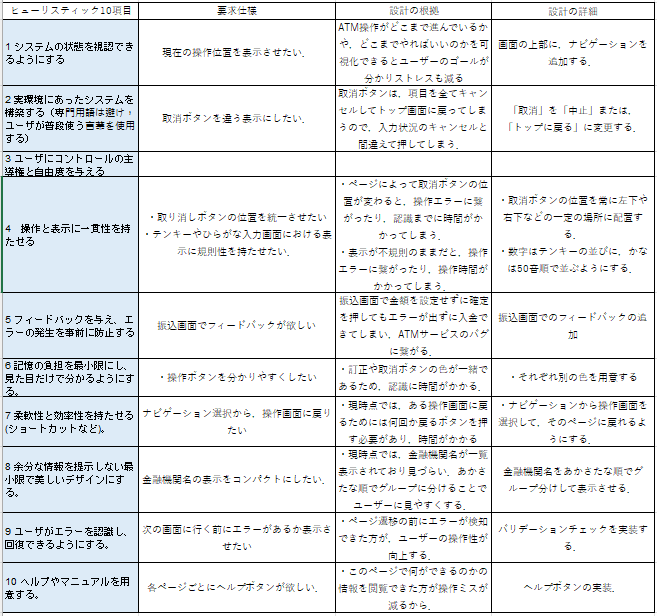
\includegraphics[width=0.8\textwidth]{image/redesign.png}
  \label{tab:redesign}
\end{table}

\section{設計の内容}
要求仕様において見た目に関する部分の優先度を高くして実装を行った.
実装画面を図\ref{fig:a_top}~図\ref{fig:m_InputError}に示す.

\begin{figure}[H]
  \centering
  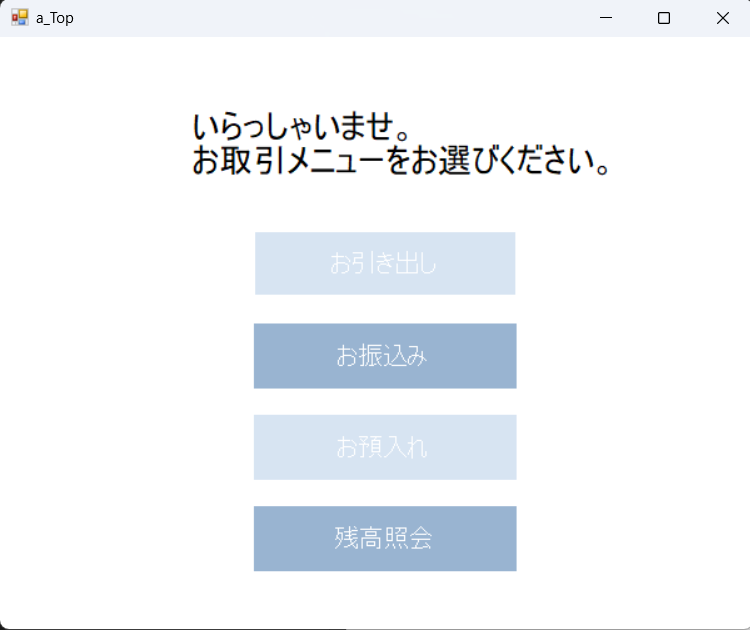
\includegraphics[width=0.7\textwidth]{image/a_top.png}
  \caption{トップ画面}
  \label{fig:a_top}

\end{figure}
\begin{figure}[H]
  \centering
  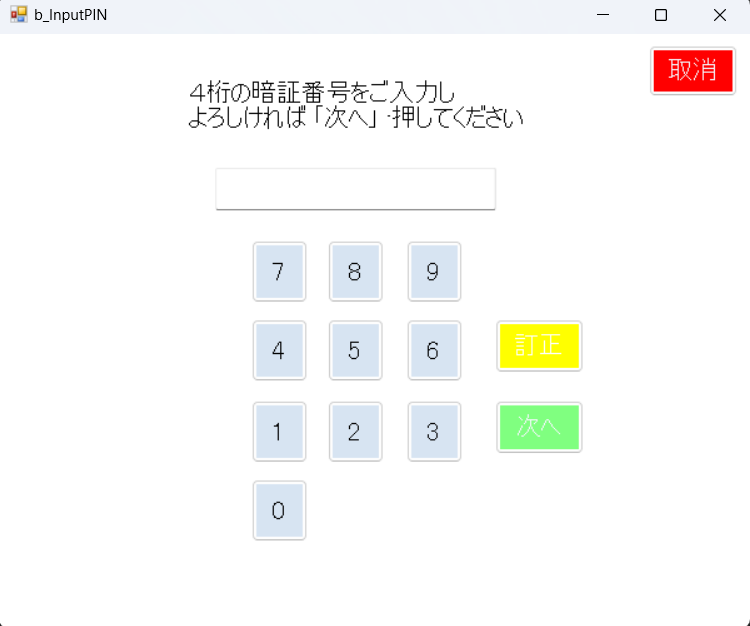
\includegraphics[width=0.7\textwidth]{image/b_inputPIN.png}
  \caption{暗証番号入力画面}
  \label{fig:b_InputPIN}
\end{figure}
\begin{figure}[H]
  \centering
  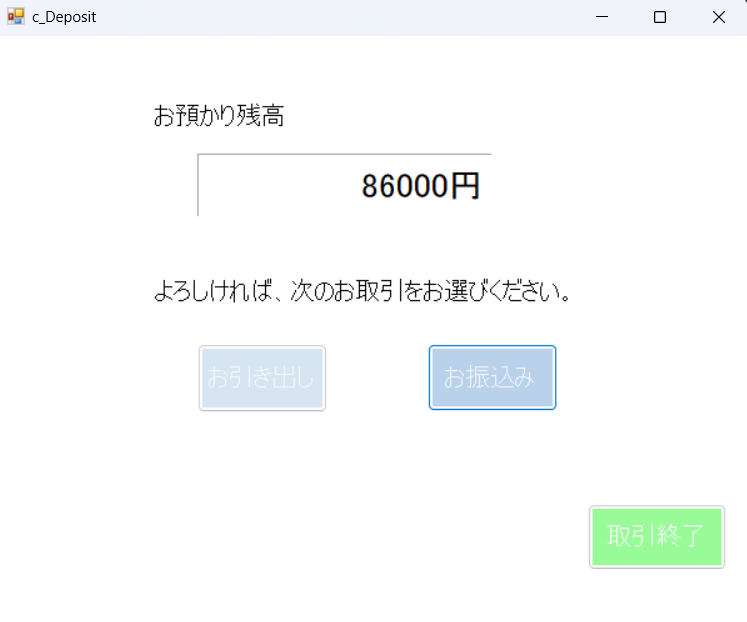
\includegraphics[width=0.7\textwidth]{image/c_Deposit.png}
  \caption{残高照会画面}
  \label{fig:c_Deposit}
\end{figure}
\begin{figure}[H]
  \centering
  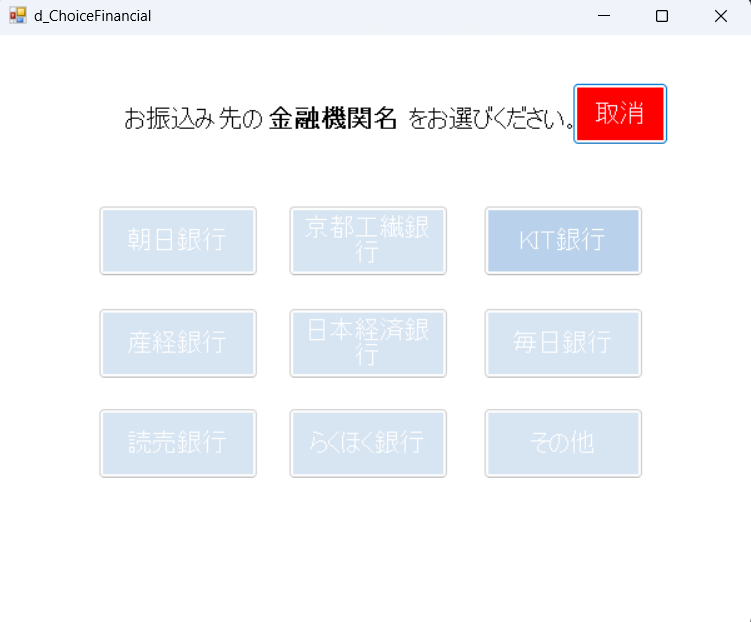
\includegraphics[width=0.7\textwidth]{image/d_ChoiceFinancial.png}
  \caption{金融機関名選択画面}
  \label{fig:d_ChoiceFinancial}
\end{figure}
\begin{figure}[H]
  \centering
  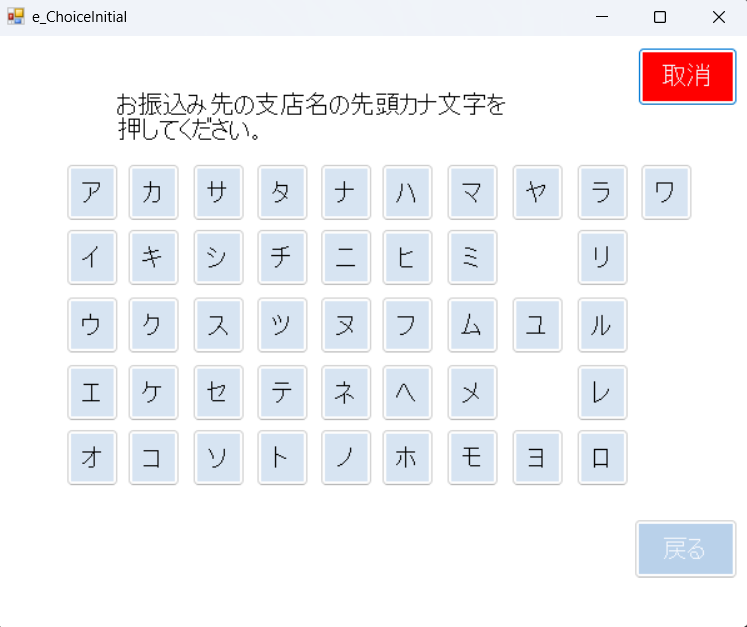
\includegraphics[width=0.7\textwidth]{image/e_ChoiceInitial.png}
  \caption{支店名の先頭文字選択画面}
  \label{fig:e_ChoiceInitial}
\end{figure}
\begin{figure}[H]
  \centering
  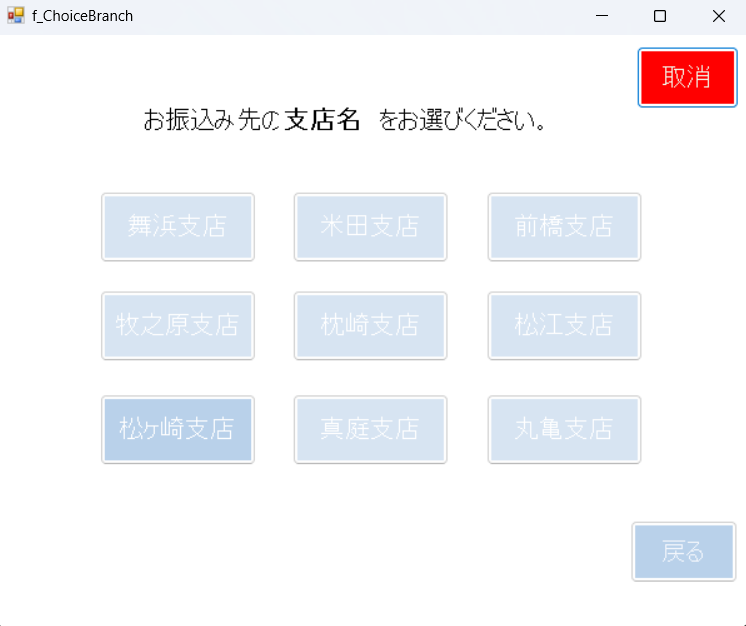
\includegraphics[width=0.7\textwidth]{image/f_ChoiceBranch.png}
  \caption{支店選択画面}
  \label{fig:f_ChoiceBranch}
\end{figure}
\begin{figure}[H]
  \centering
  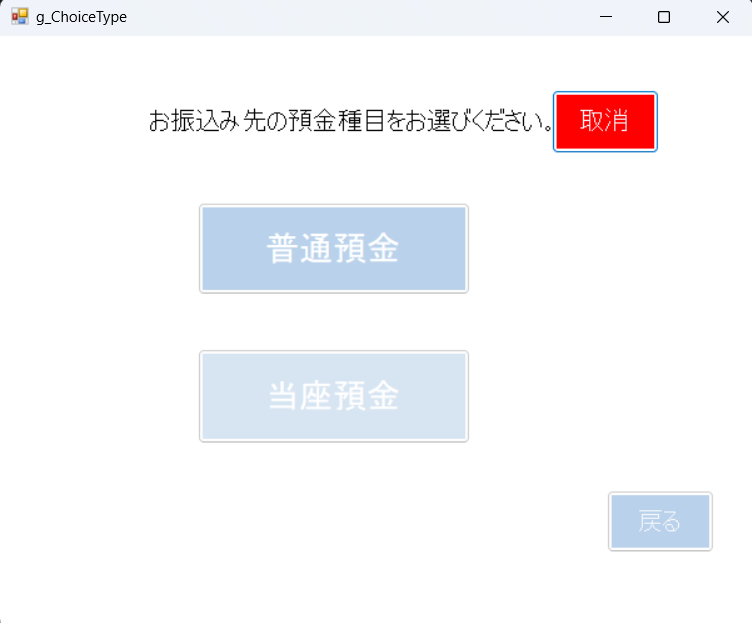
\includegraphics[width=0.7\textwidth]{image/g_ChoiceType.png}
  \caption{預金種目選択画面}
  \label{fig:g_ChoiceType}
\end{figure}
\begin{figure}[H]
  \centering
  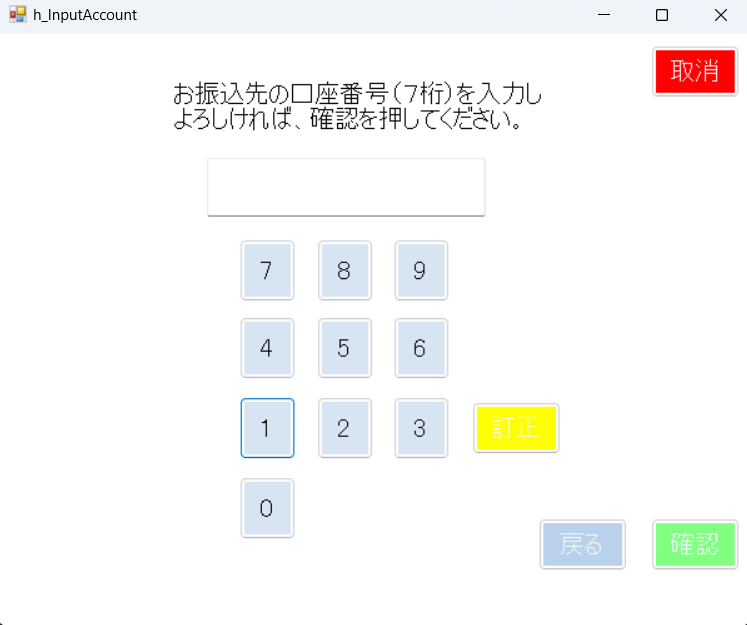
\includegraphics[width=0.7\textwidth]{image/h_InputAccount.png}
  \caption{口座番号入力画面}
  \label{fig:h_InputAccount}
\end{figure}
\begin{figure}[H]
  \centering
  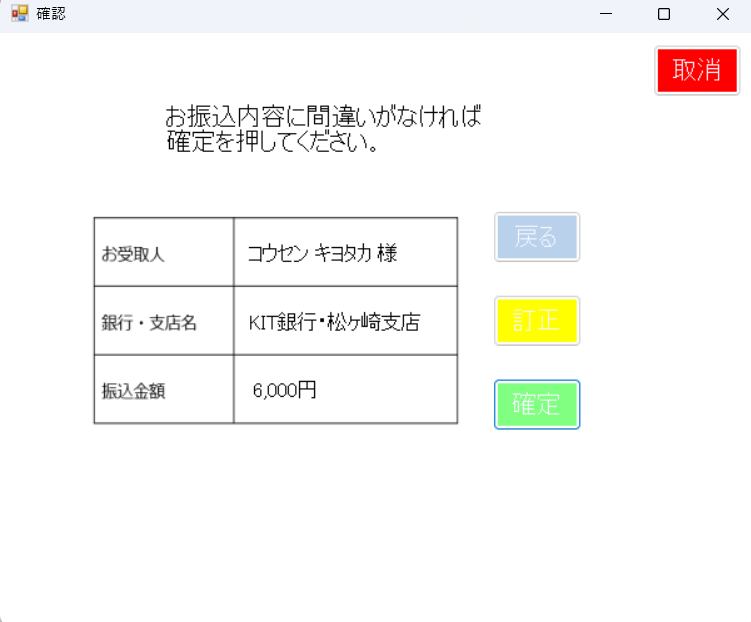
\includegraphics[width=0.7\textwidth]{image/j_Confirm.png}
  \caption{確認画面}
  \label{fig:j_Confirm}
\end{figure}
\begin{figure}[H]
  \centering
  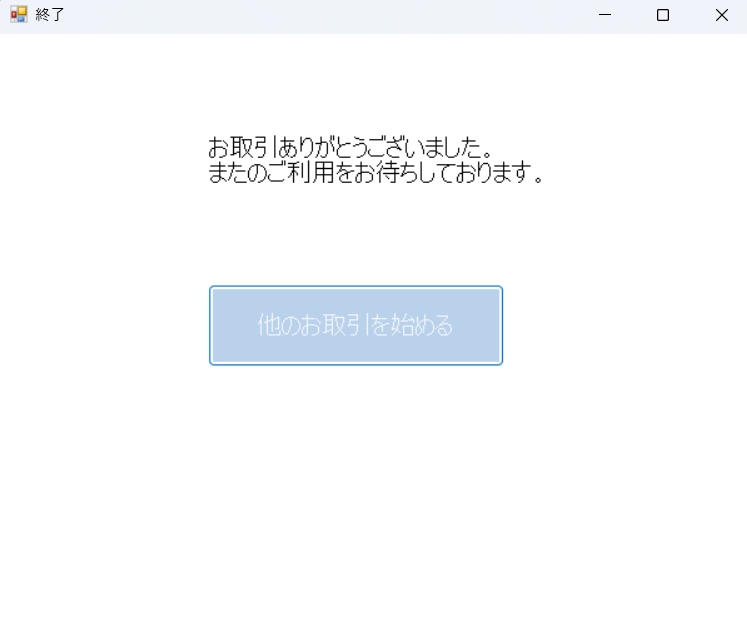
\includegraphics[width=0.7\textwidth]{image/k_Thanks.png}
  \caption{完了画面}
  \label{fig:k_Thanks}
\end{figure}
\begin{figure}[H]
  \centering
  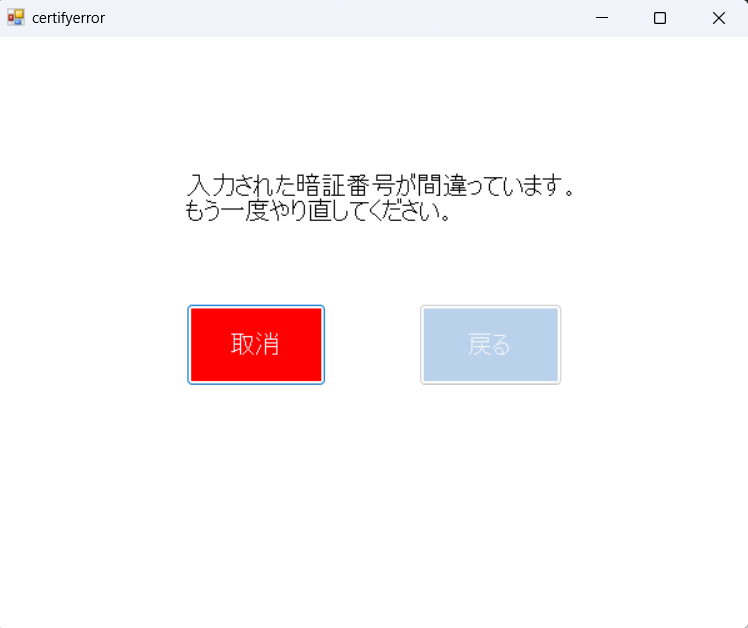
\includegraphics[width=0.7\textwidth]{image/l_CertifyError.png}
  \caption{暗証番号の誤り}
  \label{fig:l_CertifyError}
\end{figure}
\begin{figure}[H]
  \centering
  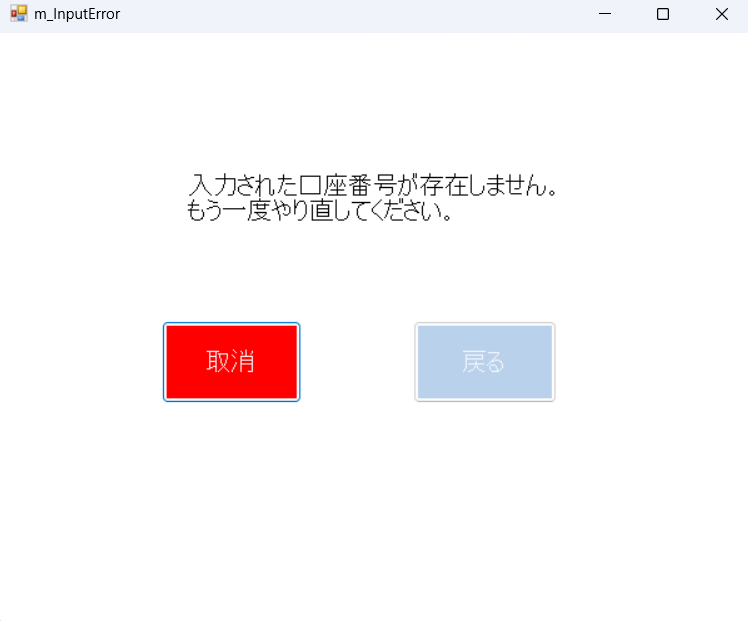
\includegraphics[width=0.7\textwidth]{image/m_InputError.png}
  \caption{口座番号の誤り}
  \label{fig:m_InputError}
\end{figure}
\begin{figure}[H]
  \centering
  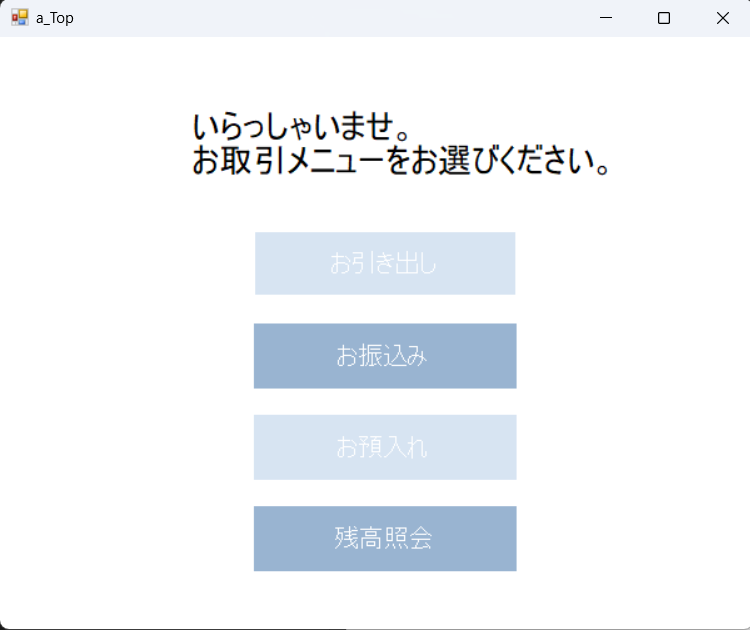
\includegraphics[width=0.7\textwidth]{image/a_top.png}
  \caption{トップ画面}
  \label{fig:a_top}
\end{figure}

\begin{thebibliography}{9}
  \item 西崎友規子.プロジェクト実習Ⅰ ヒューマンインターフェース 実験テキスト.京都工芸繊維大学,2024年
\end{thebibliography}

\end{document}